\documentclass[final,paperwidth=36in,paperheight=45in]{baposter}

\usepackage{amsmath}
\usepackage{amssymb}
\usepackage{amsthm}
\usepackage{cleveref}
\usepackage{enumitem}
\usepackage{graphicx}
\usepackage{siunitx}
\usepackage{tinos}

\begin{document}

\definecolor{white}{rgb}{1,1,1}
\definecolor{black}{rgb}{0,0,0}
\definecolor{umd-yellow}{rgb}{1,0.8509,0}
\definecolor{umd-red}{rgb}{1,0,0.1843}
\definecolor{light-gray}{rgb}{0.9,0.92,0.97}

\newcommand{\mat}[1]{\boldsymbol{#1}}
\renewcommand{\refname}{}

\begin{poster}
  {
    bgColorOne=white,
    bgColorTwo=white,
    borderColor=black,
    headerColorOne=umd-yellow,
    headerColorTwo=umd-red,
    headerborder=none,
    headershape=roundedright,
    headerfont=\Large\textsc,
    textfont=\normalsize,
    textborder=none,
    boxshade=plain,
    boxColorOne=light-gray
  }
  {
    \includegraphics[height=7em]{umd-ball.jpg}
  }
  {
    \textsc{A Radiosity Method for Thermal Modeling of Asteroids}\vspace{0.5em}
  }
  {
    Samuel F. Potter (\texttt{sfp@umiacs.umd.edu}) and Erwan Mazarico (Code 698)
    
  }
  {
    \includegraphics[height=7em]{nasa_logo.png}
  }

  \headerbox{Problem}{name=problem,column=0}
  {
    Knowledge of the illumination conditions and thermal environment
    of airless bodies is fundamental to understanding the evolution of
    their surfaces and the volatile species they may host. Permanent
    shadow exists at the Moon, Mercury, and Ceres, resulting in
    extensive cold-trapping regions which have been shown to host
    volatiles, particularly water, to varying degrees. With the
    continued exploration of small bodies, from near-Earth
    asteroids to Martian moons and to comets, we want to have the
    capability to faithfully model their thermal environment.  While
    previous modeling efforts have focused on raytracing and
    horizon-based approaches, we apply the radiosity method, first
    developed in the 90’s in the computer graphics community, to solve
    for multiple orders of scattering. The method is ideally suited to
    the application and can benefit from advances in computing since
    its development. We present the method and its implementation in
    C++, and illustrate its use with results of average incident flux
    and surface temperatures for (4) Vesta.
  }

  \headerbox{The Radiosity Method}{name=radiosity,column=0,below=problem}
  {
    \subsection*{Formulation}

    On a surface $S$, the radiosity equation is:
    \begin{equation}\label{eq:radiosity-integral-equation}
      B(x) = E(x) + \rho(x) \int_S G(x, y) B(y) dA
    \end{equation}
    where, at a point $x$ on $S$, $B(x)$ is the radiosity in
    \si{\watt\per\square\metre}, $E(x)$ is the emitted radiosity,
    $\rho(x)$ is the albedo, and $G(x, y)$ is the geometric
    kernel~\cite{cohen2012radiosity}. We discretize $S$ into a
    triangle mesh and perform a boundary element discretization (using
    point collocation) of \cref{eq:radiosity-integral-equation} to get
    the system:
    \begin{equation}\label{eq:radiosity-matrix-equation}
      \mat{K} \mat{B} = \mat{E}
    \end{equation}
    where $\mat{K}_{ij} = 1 - \rho_i \mat{F}_{ij}$, and:
    \begin{equation}
      \mat{F}_{ij} = \frac{A_j \max(0, \vec{n}_i \cdot \vec{n}_{ij}) \max(0, \vec{n_j} \cdot \vec{n}_{ji})}{\pi \|\vec{r_{ij}}\|^2}
    \end{equation}
    is the form factor matrix. The Neumann series:
    \begin{equation}
      \mat{B} = {(\mat{I} - \mat{\rho} \mat{F})}^{-1} \mat{E} = \mat{E} + \mat{\rho} \mat{F} \mat{E} + \mat{{(\rho \mat{F})}}^2 \mat{E} + \cdots
    \end{equation}
    has a simple interpretation as the direct radiosity, plus singly,
    doubly, and higher-order scattered radiosity.

    \subsection*{Solution}
    
    The dense kernel matrices arising from boundary element
    discretizations are usually very well conditioned, and iterative
    solvers typically converge in a small number of steps. To solve
    \cref{eq:radiosity-matrix-equation}, we use a Gauss-Seidel
    iteration for simplicity and implementation convenience:
    \begin{equation}
      \mat{L} \mat{B}_{n+1} = \mat{E} - \mat{U} \mat{B}_n
    \end{equation}
    Here $\mat{K} = \mat{L} + \mat{U}$, where $\mat{U}$ is strictly
    upper triangular. Approaches such as the Southwell iteration and
    progressive radiosity are other possibilites for solving
    \cref{eq:radiosity-matrix-equation}.

    \subsection*{Thermal Model}

    \vspace{-1em}

    Using the above approach, in addition to luminary radiosity, we
    drive a thermal model to simulate heat and thermal radiosity. Each
    face has an independent heat model with 17 depth layers which is
    driven using a Crank-Nicolson iteration~\cite{schorghofer-pcc}.  }

  \headerbox{Implementation}{name=implementation,column=1}
  {
    \subsection*{Flow Diagram}
    \begin{center}
      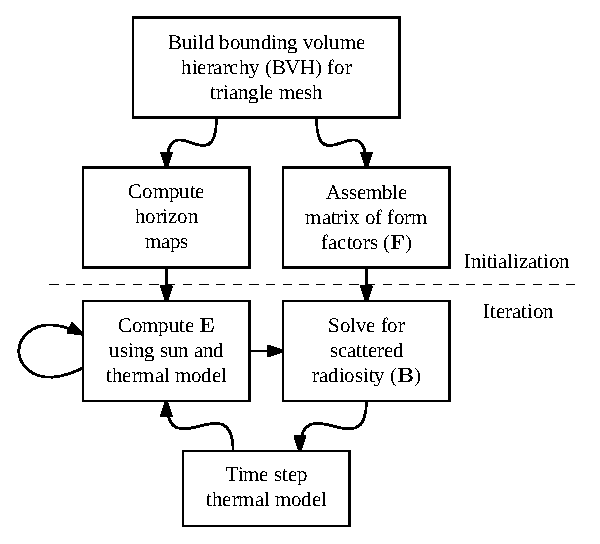
\includegraphics[width=\linewidth]{flow-diagram.eps}
    \end{center}

    \vspace{-4em}

    \subsection*{Details}
    \begin{itemize}[noitemsep]
    \item Current prototype written in C++ using Armadillo
    \item CPU parallelization of everything except G-S using Intel TBB
    \item Fast bounding volume hierarchy using SIMD
    \item Thermal model in Fortran 90~\cite{schorghofer-pcc}
    \item Plans to move to Intel MKL to scale to a cluster
    \end{itemize}
  }

  \headerbox{Numerical Results}{name=results,column=1,below=implementation}
  {
    To justify the radiosity method, we ran a battery of tests on a
    workstation with an 8-core Intel i7 processor running at 4GHz and
    with 64GB of RAM. We measured the accuracy and speed of the
    Gauss-Seidel iteration and tabulated statistics regarding the
    sparsity of $\mat{K}$. The number of nonzero elements of $\mat{K}$
    grows quadratically but with an extremely small constant. We can
    also see that the Gauss-Seidel iteration converges in
    approximately six steps independent of the model size.
    \begin{center}
      \includegraphics[width=\linewidth]{stats.pdf}
    \end{center}
    \vspace{0.03em}
  }

  \headerbox{Visualized Output: 4 Vesta}{name=visualized-output,column=2}
  {
    \includegraphics[width=\linewidth]{rad.png}
    \includegraphics[width=\linewidth]{diff_rad_avg.png}
    \includegraphics[width=0.495\linewidth]{therm_avg.png}
    \includegraphics[width=0.495\linewidth]{therm_max.png}
    \includegraphics[width=0.495\linewidth]{diff_therm_avg.png}
    \includegraphics[width=0.495\linewidth]{diff_therm_max.png}
    \vspace{-1.2em}
  }

  \headerbox{References}{name=references,column=2,below=visualized-output}
  {
    \vspace{-1.5em}
    \bibliographystyle{plain}
    \bibliography{poster} 
  }
  
\end{poster}
  
\end{document}

%%% Local Variables:
%%% mode: latex
%%% TeX-master: t
%%% End:
